\documentclass[12pt]{article}
\usepackage[utf8]{inputenc}
\usepackage[round]{natbib}
\usepackage[top=0.6in, bottom=0.6in, left=0.7in, right=0.7in]{geometry}
\bibliographystyle{plainnat}
\usepackage{graphicx}
\usepackage{float}
\usepackage{hyperref}
\usepackage{algorithm, algorithmic}
\usepackage[nottoc,notlot,notlof]{tocbibind}

\graphicspath{{images/}}

\newcommand{\ar}{\(\Rightarrow\)}
\newcommand{\pbreak}{\vspace{4mm}}

\title{\rule{\linewidth}{2pt}\\\vspace{2mm}
Project Report : CS3543 - Computer Networks 2\\
\textbf{Mini-Nmap}\\
\rule{\linewidth}{2pt}}
\author{Harsh Agarwal\\\texttt{cs15btech11019}
\and
S. Vishwak\\\texttt{cs15btech11043}}
\date{}

\begin{document}
\maketitle
\nocite{*}

\tableofcontents
\newpage

\section{Objective and Motivation}
\href{https://nmap.org/}{Nmap} has been a very-effective tool for network discovery and security analysis for about 20 years now. The goal of the project was to implement certain network discovery techniques which are available in Nmap. A full implementation of Nmap would take quite a long time of development, hence in this project, we have decided to stick with certain techniques that are popularly used.
\pbreak

The motivation of the project was to get an idea of how such network discovery tools are implemented, and to objectively see how hard implementing a suite like Nmap would actually be.

\section{Project Specifications}
The size of the project stands at around 2000 lines of code written in C++ and Python. The tools implemented as a part of the project are:
\begin{itemize}
    \item Host discovery utility
    \item Port scanning techniques: \texttt{SYN}, \texttt{FIN}, \texttt{NULL}, \texttt{XMAS} and \texttt{Decoy} scan
    \item A TCP sniffer
    \item ARP Poisoner (with ARP Doctor)
%    \item Port scanning detection using a firewall.
\end{itemize}

A full documentation of the code is available to be auto-generated for user convenience. This is discussed later.

\section{Code Structure, Design Decisions and Tools used}
\subsection{Code Structure and Organization}
The code is organized in the following manner:
\begin{itemize}
    \item \texttt{ping.h/.cpp} consists of ICMP ping preliminaries required for the host discovery.
    \item \texttt{discover.h/.cpp} consists of code required for host discovery using ICMP messages.
    \item \texttt{packet.h/.cpp} consists of code which enables socket creation, packet processing (e.g., checksum calculation), layer-wise packet assembly.
    \item \texttt{scan.h/.cpp} consists of code required for scanning techniques.
    \item \texttt{sniff.h/.cpp} consists of code required for the TCP sniffing utility
    \item \texttt{error.h/.cpp} consists of error handling utilities.
    \item \texttt{logger.h/.cpp} consists of logging utilities.
    \item \texttt{arpPoison.py} is a Python module consists of code required for a Man-in-the-Middle Attack using ARP poisoning.
\end{itemize}

\subsection{What happens in each of the files above?}
\subsubsection{\texttt{discover.h/.cpp}}
The main host discovery takes place with the \texttt{discover\_host()} function. The algorithm followed by the function is as follows:
\begin{algorithm}
\caption{Algorithm for Round-Robin based host discovery}
\begin{algorithmic}[1]
\STATE Get CIDR string and validate CIDR
\STATE \texttt{IPaddr}, \texttt{Mask} = \texttt{CIDR\_string}
\STATE Get list of \texttt{IPaddr}s using \texttt{IPaddr} and \texttt{Mask}
\STATE Populate a \texttt{Queue} with requests
\STATE \texttt{active} = \(\phi\)
\WHILE{\texttt{Queue} \(\neq \phi\)}
\STATE Open request and get the \texttt{IPaddr}
\STATE Ping the \texttt{IPaddr} and await reply
\IF{Reply received}
\STATE If \texttt{IPaddr} replies, \texttt{active} = \texttt{active} \(\cup \texttt{ IPaddr}\)
\ELSE
\STATE If non-zero trials for the request left, add to the queue. Otherwise, don't.
\ENDIF
\ENDWHILE
\RETURN \texttt{active}
\end{algorithmic}
\end{algorithm}

\subsubsection{\texttt{packet.h/.cpp}}
This a utility file. This helps create socket descriptors, assemble packets at a header level (\texttt{TCP}, \texttt{IP}), and calculate checksums.
\pbreak

The source code has been adapted and modified to requirements based on other code available online (Linux kernel). These links are available in the references and the function descriptions.

\subsubsection{\texttt{ping.h/.cpp}}
This is a utility file to handle \texttt{ICMP} packets. This file consists of functions to create sockets, assemble \texttt{ICMP} packets, and handling sending and receiving of ping messages.

\subsubsection{\texttt{scan.h/.cpp}}
Here is where the port scanning techniques take place. The most important function is \texttt{scan}. Here, too, we follow a round robin approach with requests, hence the algorithm is very similar to that specified above. Instead of \texttt{CIDR}, we will instead have a user specified range of ports, and instead of pinging we would be sending specialized packets pertaining to each technique. We have incorporated parallelism by chunking the ports to be scanned evenly across multiple threads. The scanning techniques are briefly explained below:

\begin{itemize}
    \item \underline{\texttt{SYN} Scan:} In SYN scanning, the attacking client attempts to set up a \texttt{TCP/IP} connection with a server at every possible port. This is done by sending a \texttt{SYN} (synchronization) packet, to mimic initiating a three-way handshake, to every port on the server. If the server responds with a \texttt{SYN/ACK} (synchronization acknowledged) packet from a particular port, it means the port is open. If the server responds with a \texttt{RST} (reset) packet from a particular port, it means the port is closed.
    
    \item \underline{\texttt{FIN} Scan:} In FIN scanning, the specifications of RFC 793 are exploited. RFC 793 states that: ``Traffic to a closed port should always return \texttt{RST}'' and ``If neither of the \texttt{SYN} or \texttt{RST} bits is set then drop the segment and return''. Now, if you send a packet with a \texttt{FIN} bit set to 1, then for closed ports you will receive a \texttt{RST}, but for open ports / filtered ports you will not receive anything. Thus, if there is no firewall, then there is a good chance that timeout indicates activity of the port.
    
    \item \underline{\texttt{NULL, XMAS}:} Both these work in the same way as FIN Scan, thereby exploiting the specifications of RFC 793.
    
    \item \underline{\texttt{Decoy} Scan:} To prevent a filtering of the attacker's side, there is a utility called Decoy Scan. This sends spoofed packets mimicking random \texttt{IP} address to the victim \texttt{IP} address, thus making it hard to pinpoint the attacker.
\end{itemize}

\subsubsection{\texttt{sniff.h/.cpp}}
This is a sniffing utility. Sent and Received packets are analyzed in a \texttt{process\_packet} function. This sniffer only analyzes \texttt{TCP} packets, since most of our scans are designed to work with the \texttt{TCP} header.

\subsubsection{\texttt{arpPoison.py}}
This has two key functions - \texttt{poisoner} and \texttt{doctor}. \texttt{poisoner} will tell the victim that the MAC address of the gateway is its own, and will tell the gateway that the victims's MAC address is its own. Now packets inbound to the victim from anywhere will be intercepted by the attacker.
Messages from the victim to the gateway, will be intercepted by the attacker as well.
\pbreak

To revert the changes made, the "doctor" broadcasts messages as the gateway and victim asking for the MAC addresses of the victim and gateway respectively, thus restoring the ARP tables.
\pbreak

This is a simple man-in-the-middle attack, which is why we decided to add it in this suite. The network library ScaPy was used for this module alone. The main file will execute the attack for a given duration, after which the attacked reprises the role of a "doctor" and reverts the changes

\subsection{Design Decisions}
Certain design decisions were made as a part of the project. We chose C++ over Python, despite the huge module support from Python, since we believed that C++ was closer to the Linux Network API than Python, thus  leaving room for less error. We have also made use of threads for parallel port scanning, and Python's threading module is not as efficient as C++, which is also another reason to migrate to C++.
\pbreak

However, for the ARP poisoning tool, we decided to go with Python instead of C++, since it would require dealing with the link-layer packets, which could cause a lot of pointer manipulation, which is tedious and error-prone.
\pbreak

We have also effectively modularized our code, so that the utilities designed could also be used for other purposes than their intended usage as well. For example, we have a ICMP message sender which can be used in place of the \texttt{iputils} utility \texttt{ping}.
\pbreak

In the host discovery and port scanning techniques, we have decided to use a Round-robin technique. Here, we create a queue of ``requests'', and these ``requests'' are processed in a round-robin fashion. If a ``request'' is successfully completed or has run out of trials, then we remove it from the queue. Other alternatives were to wait until a reply arrived for a given request - which is susceptible to timeouts. This round-robin scheme allows us to pipeline the process as well.
\pbreak

We have also made use of raw sockets (specified using \texttt{SOCK\_RAW}). This helps us modify the properties of the socket to our will (for example: sending spoofed packets), which is why we decided to use them over traditional stream or datagram sockets. Using raw sockets, we were able to populate the header appropriately as per requirements (for TCP, IP, and ICMP).

\subsection{Tools used}
\begin{minipage}{0.48\linewidth}
We have made use of \href{https://www.openstack.org/}{\texttt{OpenStack}}. Using this, we have created a private subnet, which behaves as the test-bed for our tools. The setup can be seen to the right.
\end{minipage}
\hfill
\begin{minipage}{0.48\linewidth}
\begin{figure}[H]
\centering
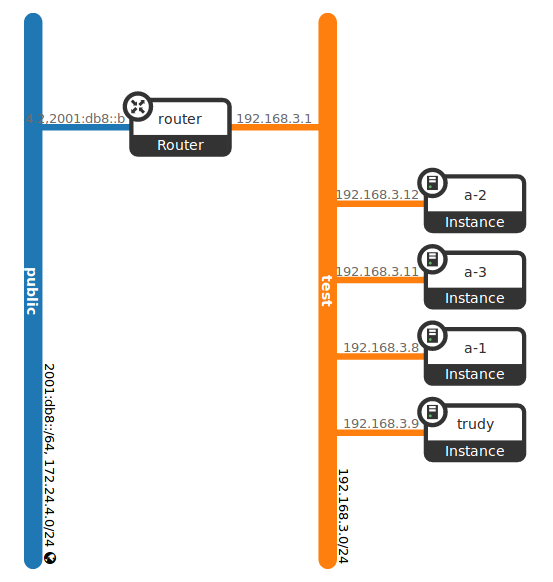
\includegraphics[width=0.75\linewidth]{open-stack-setup.png}
\end{figure}
\end{minipage}
\pbreak

We have also made use of \texttt{tcpdump} and \texttt{WireShark} for monitoring the network traffic during the time of the attack.
\pbreak

For specifying input to the executable, we have used a JSON (Javascript Object Notation) parser designed by Niels Lohmann. The file \texttt{json.h} is code for the aforementioned parser.
\pbreak

The documentation in generated using \href{http://www.stack.nl/~dimitri/doxygen/}{Doxygen}.

\section{Contributions}
Our contributions are listed below:
\begin{itemize}
    \item Port Scanning techniques and the TCP Sniffer were implemented by Harsh Agarwal.
    \item Host discovery utility and ARP Poisoner (with Doctor) were implemented by Vishwak Srinivasan.
\end{itemize}

In addition, the \texttt{OpenStack} setup was made by Harsh Agarwal.

\section{Code tutorial}
\subsection{Documentation generation}
To obtain the documentation for the project, one can go the home folder of the project, and perform
\[\texttt{make docs}\]

This will create a \texttt{docs} directory in the same directory of the project. Opening \texttt{index.html}, will help view the project from a GUI.
\begin{figure}[H]
\begin{minipage}{0.475\linewidth}
\centering
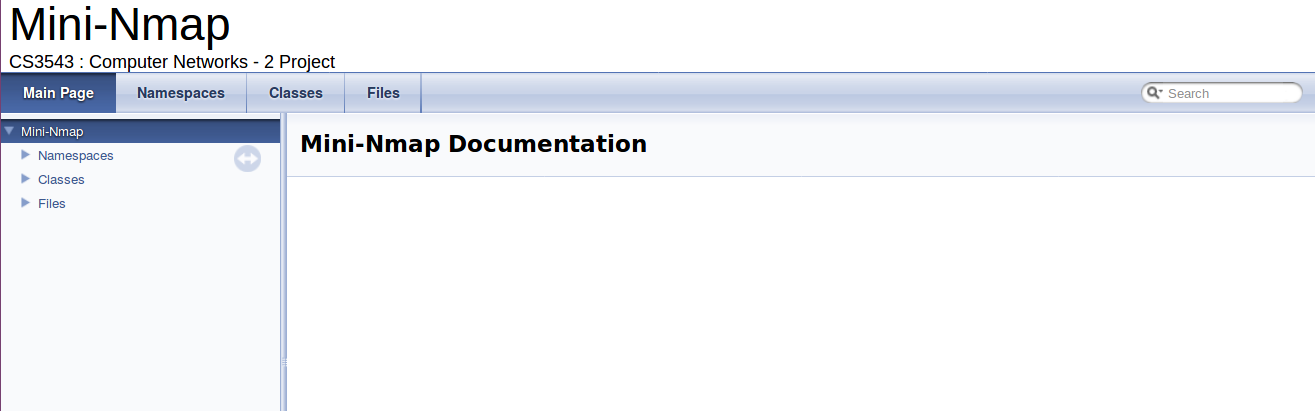
\includegraphics[width=0.9\textwidth]{doc-gen-1.png}
\caption{Home page of generated docs. View the taskbar on the left.}
\end{minipage}
\hfill
\begin{minipage}{0.45\linewidth}
\centering
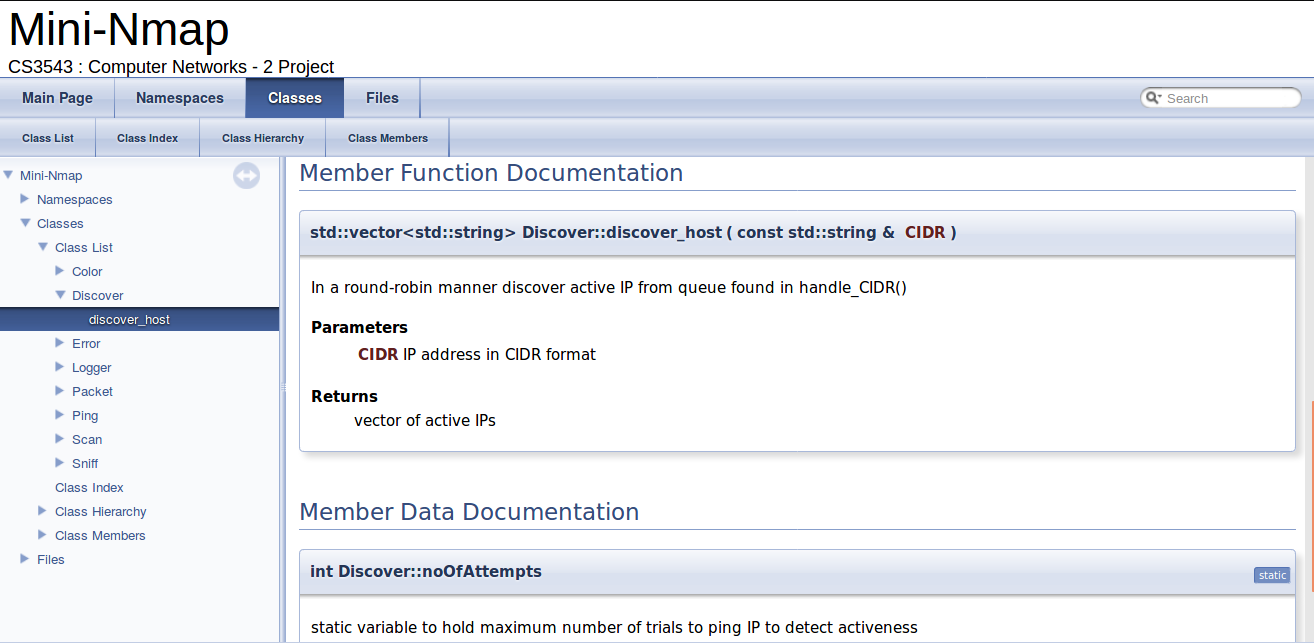
\includegraphics[width=0.9\textwidth]{doc-gen-2.png}
\caption{One can view member functions and data as well}
\end{minipage}
\end{figure}

\subsection{Building the project}
\begin{minipage}{0.475\linewidth}
\begin{figure}[H]
\centering
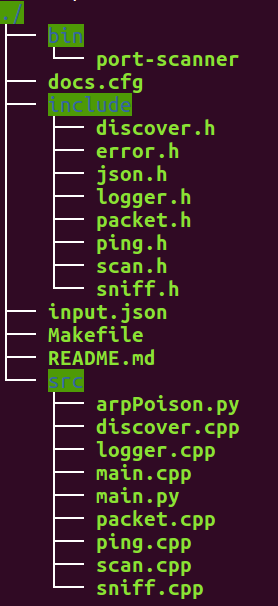
\includegraphics[width=0.6\linewidth]{file-structure-1.png}
\end{figure}
\end{minipage}
\hfill
\begin{minipage}{0.475\linewidth}
Again, using the \texttt{Makefile}, one can perform
\[\texttt{make all}\]

This will build the project. The compiled binary named \texttt{port-scanner} will be placed in \texttt{./bin}, after compilation. Note the tree structure for more information.
\end{minipage}

\subsection{Running the generated binary}
The executable takes a configuration file supplied in a JSON format, the CIDR to get the list of IPs to test for activity and the scanning technique - one of \texttt{SYN}, \texttt{FIN}, \texttt{NULL}, \texttt{XMAS} and \texttt{Decoy}, in that order.
\pbreak

\begin{minipage}{0.475\linewidth}
In the \texttt{JSON} file, you have to specify parameters based on which your port scanner will work. Beside is a sample \texttt{JSON} file. This file is also provided in the code.
\end{minipage}
\hfill
\begin{minipage}{0.475\linewidth}
\centering
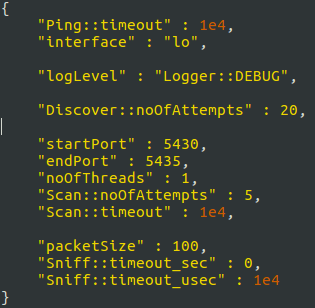
\includegraphics[width=0.9\linewidth]{sample-json.png}
\end{minipage}
\section{Results}

\subsection{\texttt{SYN} Scan}
Below is the screenshot of a \texttt{Wireshark} trace of a successful \texttt{SYN} Scan. In the first 4 packets, you can see the IP discovery utility in action. After this, the \texttt{SYN} scan starts, indicated by a number of \texttt{SYN} packets.

\begin{figure}[H]
\centering
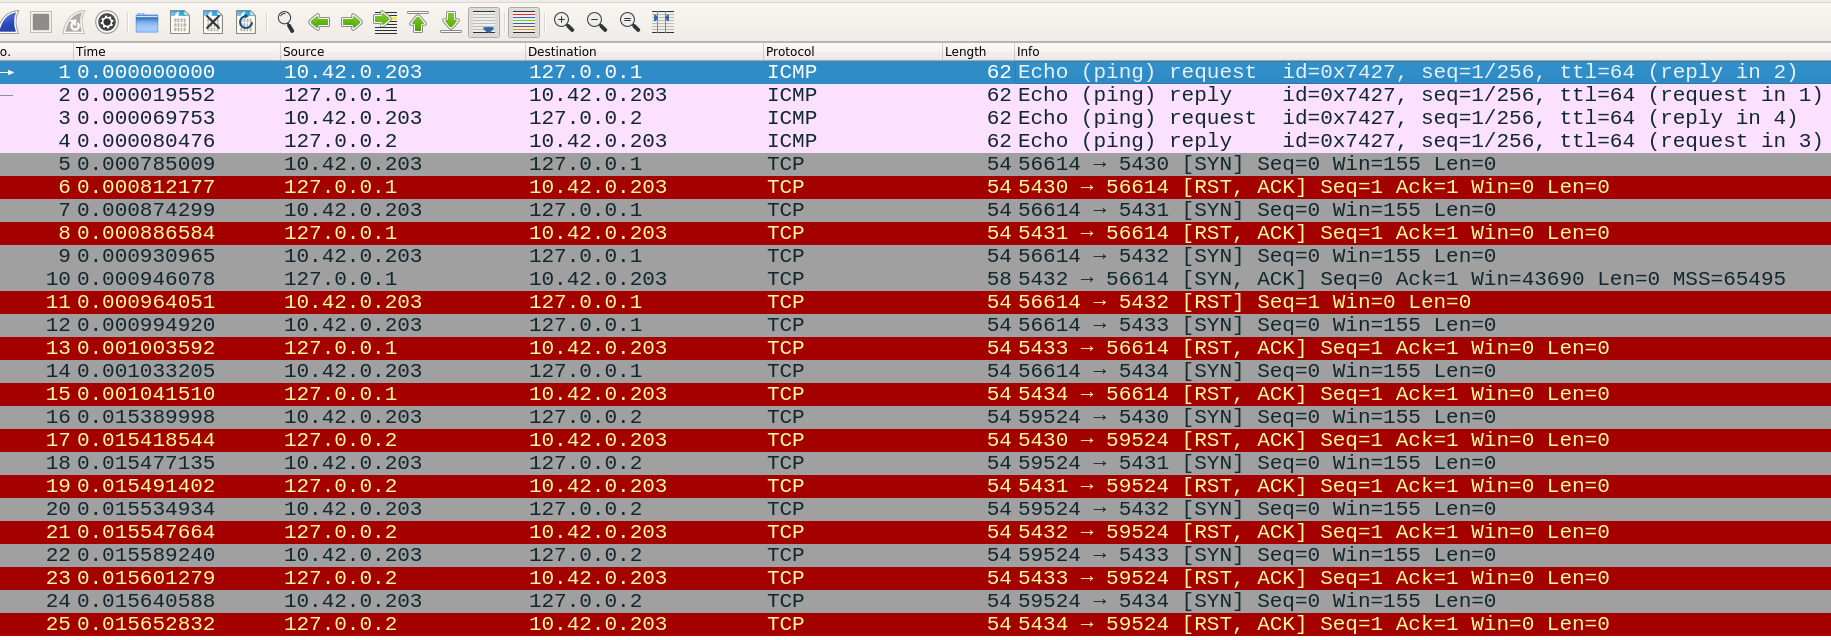
\includegraphics[width=0.75\linewidth]{syn-scan-wireshark.png}
\caption{Note that there is a \texttt{SYN/ACK} for the port 5432, which we had open in the setup.}
\end{figure}

\subsection{\texttt{XMAS} Scan}
Below are some screenshot of the testing. As specified earlier, for those ports which are either filtering / open, there will be a timeout, and the closed ports will send a \texttt{RST} no matter what. The number of trials is 5, which is why you can see 4 re-transmissions.

\begin{figure}[H]
\begin{minipage}{0.48\linewidth}
\centering
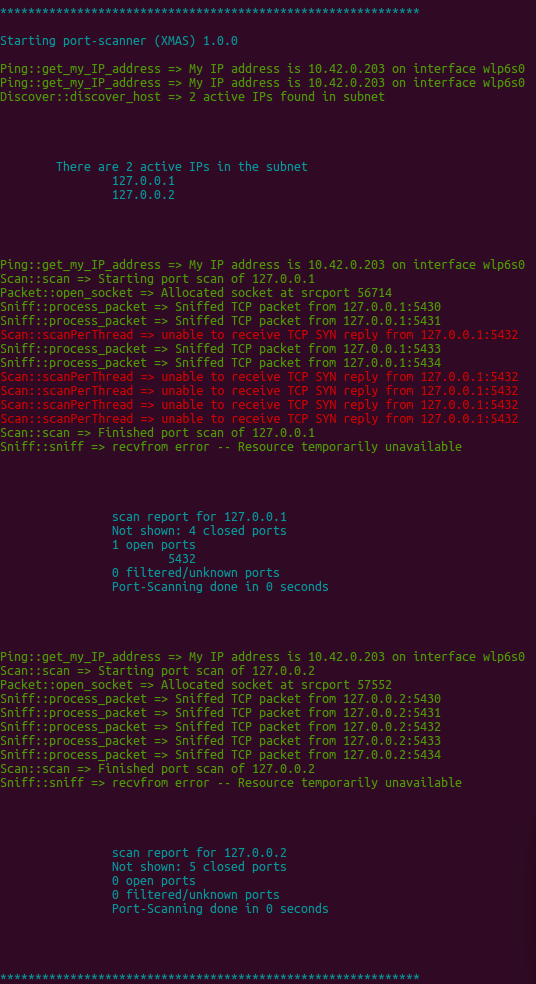
\includegraphics[width=0.65\textwidth]{xmas-output.png}
\caption{The terminal output.}
\end{minipage}
\hfill
\begin{minipage}{0.48\linewidth}
\centering
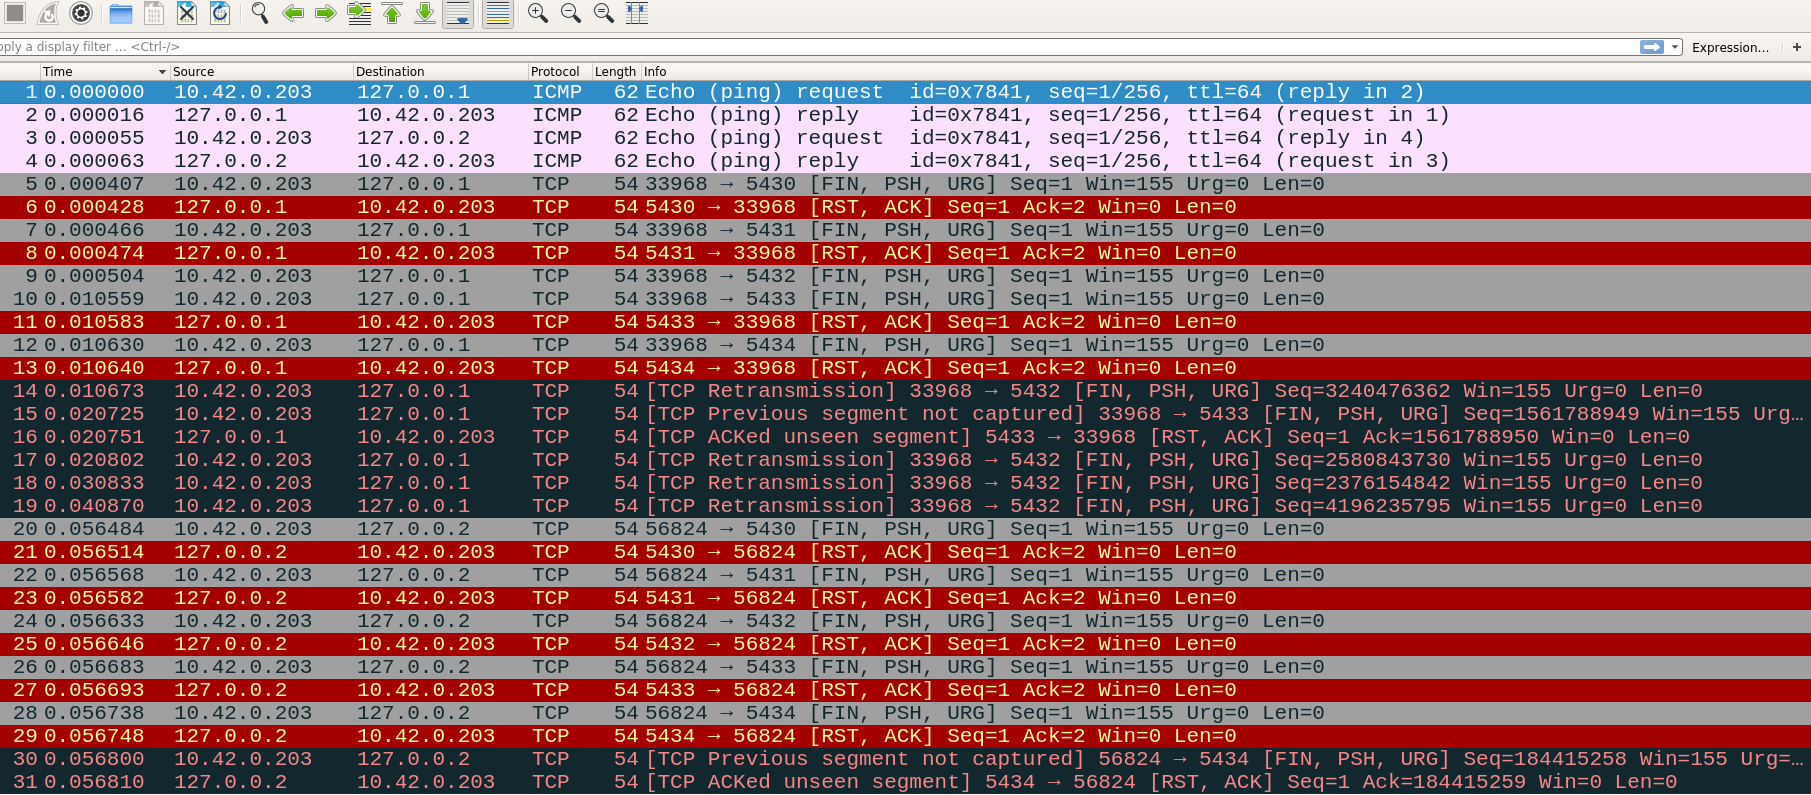
\includegraphics[width=\textwidth]{wireshark-xmas.png}
\caption{\texttt{Wireshark} output for \texttt{XMAS} scan}
\end{minipage}
\end{figure}

\subsection{\texttt{Decoy} Scan}
Below is a screenshot of the \texttt{Decoy} scan in action. Note that the IP address to which \texttt{SYN} packets are sent are not one but many, thus fooling the system. Also the \texttt{RST} is sent from the OS, which will prevent a seemingly \texttt{DOS} attack.

\begin{figure}[H]
    \centering
    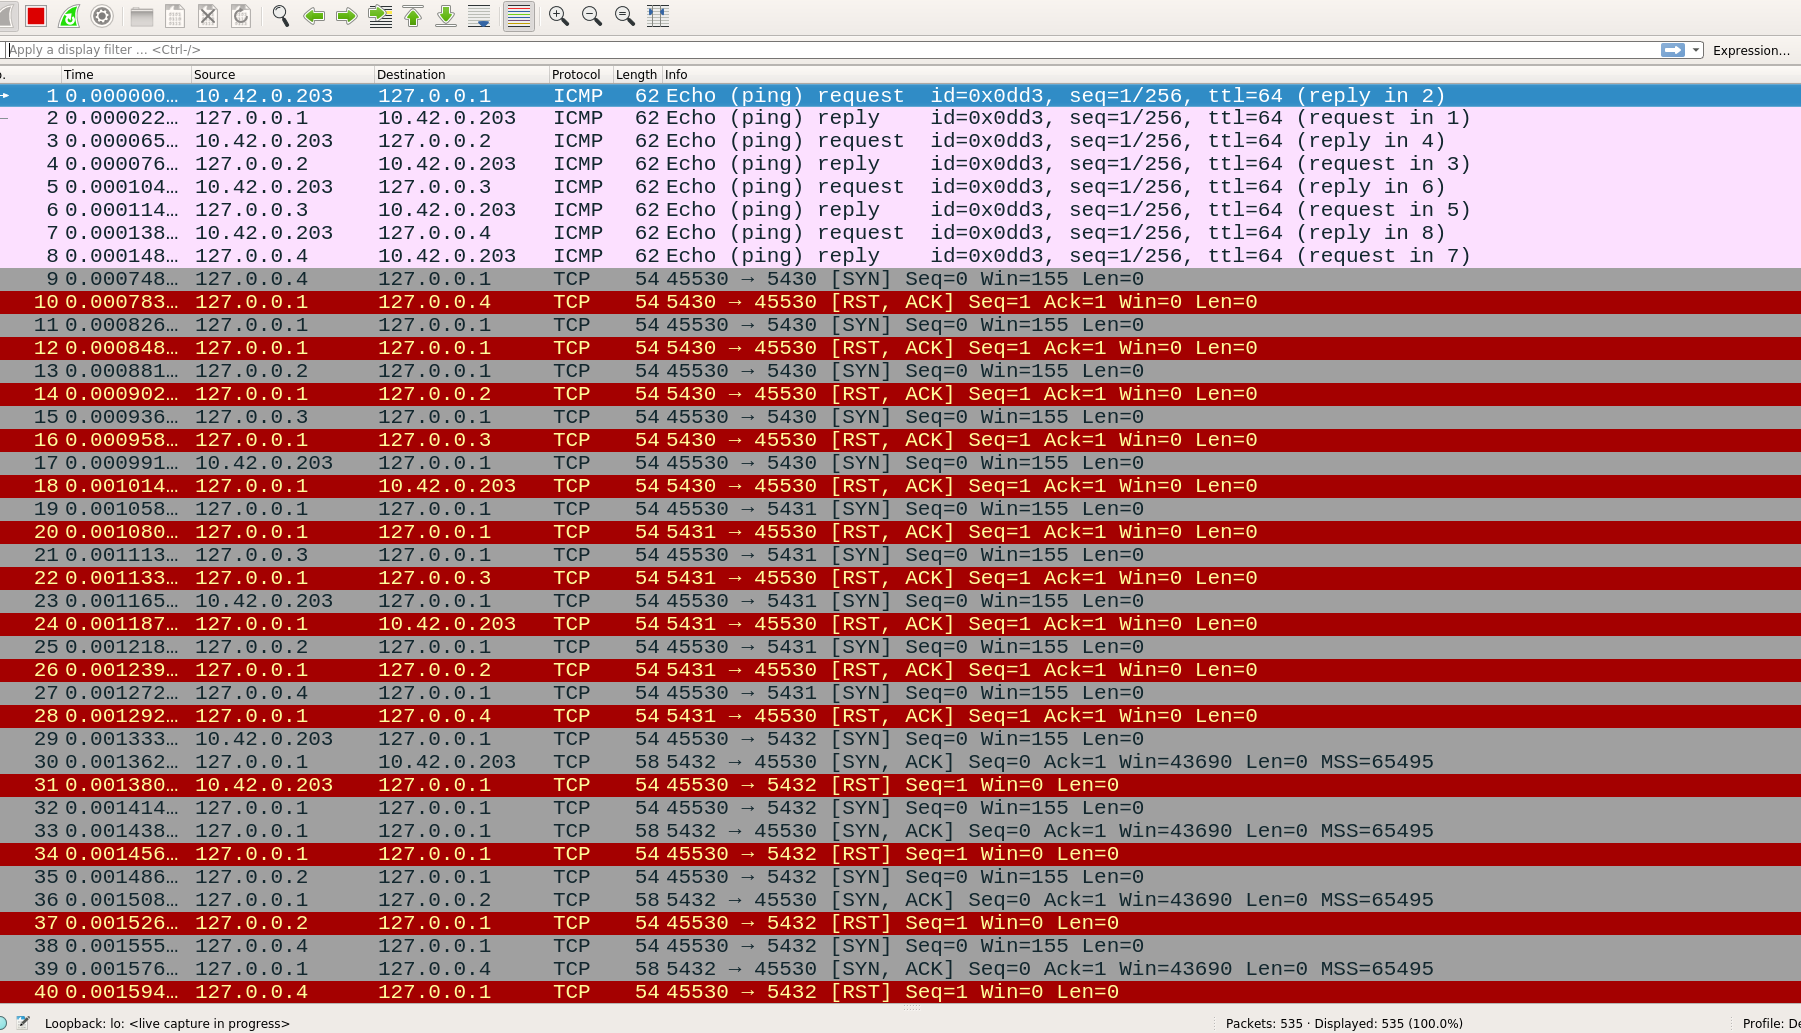
\includegraphics[width=0.75\linewidth]{decoy.png}
\end{figure}

\subsection{\texttt{ARP} Poisoner}
The poisoner successfully sends packets whilst trying to spoof the \texttt{ARP} entries. Unfortunately, these packets were not able to be detected at the hosts on \texttt{OpenStack}. Digging into the issue led us to a \href{https://specs.openstack.org/openstack/neutron-specs/specs/kilo/arp-spoof-filtering-ebtables.html}{patch} in \texttt{OpenStack} that prevents this behaviour. We didn't want to test this on a live network fearing it might cause issues to multiple-systems.
\pbreak

Below are the screenshots of the ARP Poisoner at work. These are outputs from the \texttt{tcpdump} utility:
\begin{figure}[H]
\begin{minipage}{0.475\linewidth}    
\centering
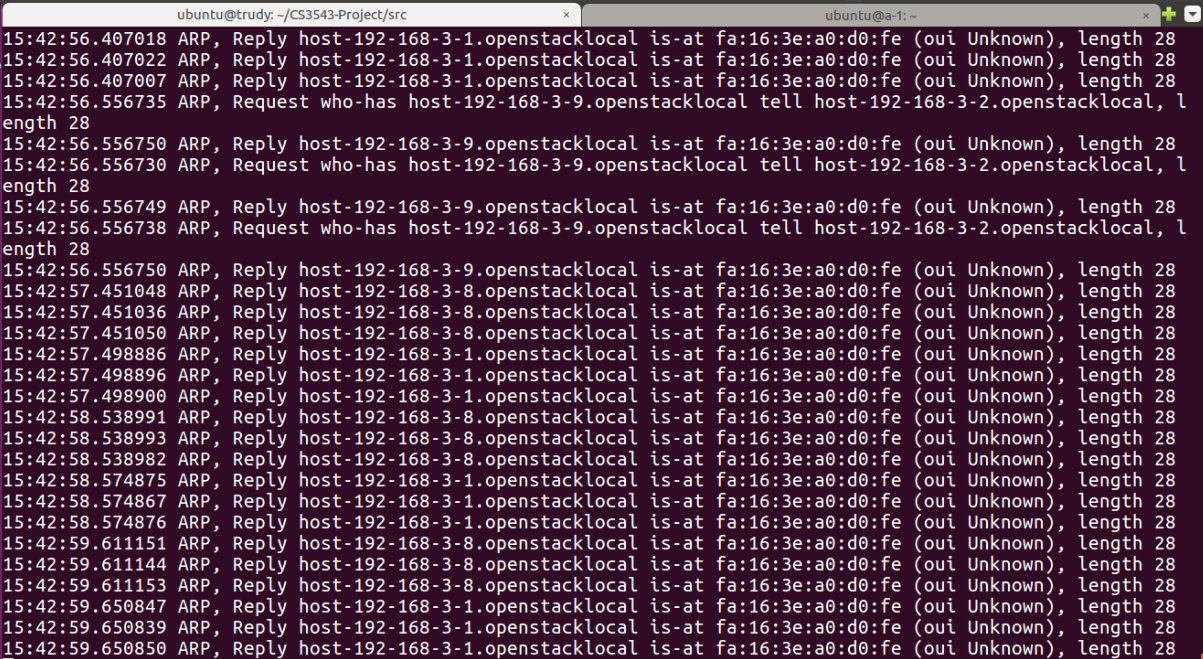
\includegraphics[width=\textwidth]{trudy-side-sending.png}
\caption{Trudy is successfully spoofing the network}
\end{minipage}
\hfill
\begin{minipage}{0.475\linewidth}    
\centering
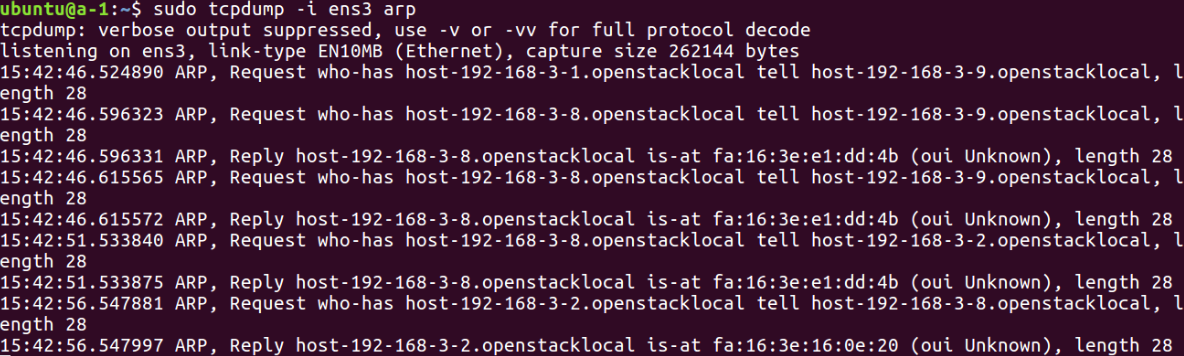
\includegraphics[width=\textwidth]{a1-side-receiving.png}
\caption{A-1 (a victim) is unable to receiving the spoofed \texttt{ARP} messages}
\end{minipage}
\end{figure}

\section{Scope for improvement}
We had a working prototype a firewall, which will be able to detect port-scanners. We were able to test it completely, which is why we haven't submitted it as a part of the project.
\pbreak

Furthermore, we also would like improve this by adding an \texttt{OS} fingerprinting technique, wherein specifics of the networking \texttt{API}s of multiple OSes are exploited to possibly find of the \texttt{OS} operating at each port.

\bibliography{main.bib}
\end{document}